\documentclass[11pt,a4paper]{article}
\usepackage[left=2.3cm,top=2cm,right=2.3cm,bottom=2.0cm]{geometry}
\usepackage{geometry}
\usepackage{amsmath}
\usepackage{amssymb}
\usepackage{txfonts}
\usepackage{microtype}
\usepackage{epsfig}
\usepackage{graphicx}
\usepackage{moreverb}
\usepackage{hyperref}
\usepackage{listings}
\usepackage{xcolor}
\usepackage{textcomp}
\usepackage{makecell}
\usepackage{wasysym}
\definecolor{listinggray}{gray}{0.98}
\definecolor{lbcolor}{rgb}{0.98,0.98,0.98}
\lstset{
	backgroundcolor=\color{lbcolor},
	tabsize=4,
	rulecolor=,
	language=matlab,
    basicstyle=\scriptsize\ttfamily,
    upquote=true,
    aboveskip={1.5\baselineskip},
    columns=fixed,
    showstringspaces=false,
    extendedchars=true,
    breaklines=true,
    prebreak = \raisebox{0ex}[0ex][0ex]{\ensuremath{\hookleftarrow}},
    frame=single,
    showtabs=false,
    showspaces=false,
    showstringspaces=false,
    identifierstyle=\ttfamily,
    keywordstyle=\color[rgb]{0,0,1},
    commentstyle=\color[rgb]{0.133,0.545,0.133},
    stringstyle=\color[rgb]{0.627,0.126,0.941},
}

\usepackage{tikz}
\usepackage{pgfplots} 
\usepackage{pgfgantt}
\usepackage{pdflscape}
\usepackage{subcaption}
\usepackage{adjustbox}
\usepackage{siunitx}
\pgfplotsset{compat=newest} 
\pgfplotsset{plot coordinates/math parser=false}
\usepackage{pdfpages}
\usepackage{placeins}
\usepackage{wrapfig}





\newlength\fwidth
\newlength\fheight
\pagestyle{myheadings}

\pgfplotsset{every axis/.append style={
        scaled y ticks = false, 
        scaled x ticks = false, 
        y tick label style={/pgf/number format/.cd, fixed, fixed zerofill,
                            int detect,1000 sep={\;},precision=3},
        x tick label style={/pgf/number format/.cd, fixed, fixed zerofill,
                            int detect, 1000 sep={},precision=3}
    }
}

\usepackage{eso-pic}
\usepackage{ifthen}

\usepackage[nottoc]{tocbibind}
\usepackage[backend=biber,style=numeric,sorting=none]{biblatex}
\addbibresource{bibben.bib}

\usepackage{float}
\usepackage{subcaption}
\usepackage{gensymb}
\usepackage{siunitx}
\usepackage{enumitem}

\title{Project 3: Approximate Bayesian Computation}
\author{
  Kevin Andersson\\
  \texttt{kevinan@student.chalmers.se}
  \and
   Eric Lindgren\\
  \texttt{ericlin@chalmers.se}
}

\markright{Kevin Andersson and Eric Lindgren, Group 7}

\begin{document}

\maketitle

\pagenumbering{gobble}% Remove page numbers (and reset to 1)
% \newpage
\pagenumbering{arabic}% Arabic page numbers (and reset to 1)
\setcounter{page}{1}
\section{Introduction and Background}

When conducting scientific experiments the end goal is always to investigate and learn something, in reality this often boils down to performing statistical inference on some parameter or models. In many cases this can however be very hard when the theory of the problem becomes very complicated. An example of this is the discovery of the Higgs boson at CERN \cite{lec13}. This process contains many different steps of theory from the probability distributions of the incoming parton momenta to different scattering channels described by the Feynman diagram to the interaction in the detectors. The problem consist of multiple unobserved latent variables and even if these would been known it is very hard to write down a likelihood of the event.

In this report we will study a much simpler problem but conceptually similar to the discovery of the Higgs boson; the modified Galton board. The Galton board is sitting on a rocking ship which gives the beads a bias of falling on a particular side of the pegs. The beads also have a sort of inertia that originate from their obtained spin after bouncing of the previous peg. The modified Galton board can be described using equation \ref{eq:galton} which describes the probability of a bead hitting a peg on the Galton board to either turn left or right. 
\begin{equation}
    \label{eq:galton}
    P_{\pm} = 0.5 \pm \left(\alpha M + s \right)
\end{equation}
$M$ here is either -0.5 or 0.5 if it bounces of to the left respective to the right of the last peg, it is  0 from start.  Since we are on a rocking ship the $s$-parameter can be seen as random and thus a latent variable, while $\alpha$ is constant. The goal thus is to perform inference on $\alpha$. This is however, as previously hinted about, very hard since it is impossible (or extermly difficult) to write down a likelihood, to resovle this we use turn to Bayesian inference which has the solution.


When performing Bayesian inference first you need some experimental data and then also a model connecting you unknown variable to the experiment by some theory. The goal is then to evaluate/sample the posterior
\begin{equation*}
    p(\theta|y_{obs}) \propto p(y_{obs}|\theta) p(\theta).
\end{equation*}
In some cases when the model is complicated it can be very hard our sometimes impossible to evaluate the likelihood, however there might be a way to, for a given set of parameters $\theta$, perform simulations. One can then evaluate the posterior by performing likelihood-free sampling. Likelihood-free sampling is based on rewriting the posterior as
\begin{equation*}
    p(\theta|y_{obs}) \propto \int d y \delta(y-y_{obs})p(y|\theta) p(\theta),
\end{equation*}
where $y_{obs}$ is some observed data. The posterior can thus be sampled by drawing $\theta^*$ from the prior $p(\theta)$, perform a simulation for $y^*  = f(\theta^*)$, and accept the sample if $y^* = y_{obs}$. This is an amazing result; we can sample the posterior even if we can't evaluate the likelihood analytically. But there might still be a crucial problem left tackle, namely that the requirement  $y^* = y_{obs}$ will give an acceptance ration equal to zero if the observed data is given by a continuous distribution of outcomes. This is also a problem the grows with the dimensionality in the observed data. The problem can be solved by Approximate Bayesian Calculation (ABC) which consists of replacing the delta function by 
\begin{equation*}
    p(\theta|y_{obs}) \propto \int d y \frac{1}{h}K\left(h^{-1}{||y - y_{obs}||}\right) p(y|\theta) p(\theta).
\end{equation*}
$K$ is the kernel satisfying $\int K(\xi)d\xi = 1$, $\int\xi K(\xi)d\xi = 0$ and $\int \xi^2K(\xi)d\xi < \infty$. $h$ is a parameter that governs the crudeness of the approximation and we see that if $h\to 0$ ABC reduces to likelihood-free sampling. $||y - y_{obs}||$ is called a summary statistic and is a measure of similarity between the observed data and the simulated data. There exists many different summery statistics and the choice is up to the one performing the sampling; note however that one should be cautious about the choice since it can greatly effect the accuracy of the sampling and one should carefully investigate the approximation errors when doing approximate inference.

Since the modified Galton board is a prime example of when we can't evaluate the likelihood ABC is very applicable to this problem. However the latent variable $s$ will make the convergence slow and the computational cost of performing ABC very high. In this report we therefore study a way of combining ABC with neural networks to eliminate this latent variable and speed up convergence. This makes it possible for us to perform the inference on $\alpha$ and in more complicated problems with more latent variable this method may be of significant importance. 

\section{Methodology}

% BEskriv modellen här - kanske plotta några simulerade distributioner? Men ha inte med det i resultatet, endast NN och ABC i resultat.

\subsection[Task 1]{Neural network as a generator of prospective samples}
\label{sec:method_NN}
One issue with ABC is that convergence can be slow \cite{rasmusbaath}. In order to remedy this, we developed a neural network to generate candidates for the parameter $\alpha$ and the latent parameter $s$, given an input distribution from the simulator. By training the network, the hope is then that the prospective parameter samples generated by the network when fed with the observed distributions from the experiments will be more likely to be accepted by the ABC algorithm than drawing samples directly from the respective parameter priors, speeding up convergence. Hence, we generated a dataset consisting of 300000 distributions $\mathbf{X}$ from the simulator, each for different input parameters $y = (\alpha, s)$. The values for $\alpha$ and $s$ where drawn uniformly randomly in the respective intervals, $\alpha\in[0, 0.5]$ and $s\in[-0.25, 0.25]$. The neural network was trained to predict the parameters $y$, given the input distributions $\mathbf{X}$ with a 70\%/30\% training/validation split. Since the parameters $y$ are continuous, this corresponds to a regression problem. The network architecture consisted of two fully connected layers, of 32 and 2 units each, and no hidden layers. The input layer was activated using the ReLU function, with no activation being applied to the output layer in order to not constrain the output of the network (due to this being a regression problem). In order to monitor the training and the performance of the network, the loss function mean absolute error (MAE) was used. The network was implemented using Keras/Tensorflow.


% \subsection[Task 4]{Approximate Bayesian Computation}
% \label{sec:method_ABC}
% Nästan så man kanske vill flytta det här till ett teoriavsnitt? 


\subsection{Application of naive ABC to a toy problem}
Now when we have a neural network able to predict $\alpha$ and $s$ from an experiment we want to use this to implement a NN aided ABC algorithm to perform inference on the $\alpha$-parameter \cite{lec3}. At hand we have a set of performed experiments all with the same but unknown $\alpha$, but all the experiments also has an independent unknown latent variable, the bias $s$. When performing ABC one would then normally draw both $\alpha$ and $s$ from a prior and accept the candidate $\alpha$ with a probability given by the kernel. However, since $s$ heavily affects the result of the experiment the acceptance ratio of the sampling would decrease dramatically. So to increase the acceptance ratio and thus speed up the convergence we use a neural network (NN) trained to determine $\alpha$ and $s$ from an experiment/simulation. We can thus instead of drawing $s$ from a prior draw it from a distribution defined by the NN prediction and its uncertainty. More precisely, we draw a $s^* \sim \mathcal{N}(s_m, \sigma_s)$, where $s_m$ is the prediction from the NN for $y_{obs}$ and $\sigma_s$ is the standard deviation in the predictive $s$ error for some simulated validation data. Our sampling of the posterior can then be summarized by the following algorithm. 
\begin{enumerate}
    \item $y_{obs} \mapsto \alpha_m, s_m$
    \item $s^* \sim \mathcal{N}(s_m, \sigma_s)$
    \item $\alpha^* \sim \pi(\alpha)$
    \item perform simulation $y = f(\alpha^*, s^*)$
    \item accept with probability $K(h^{-1}||y - y_{obs}||)$
    \item repeat 2-4
    \item repeat 1-6 for all $y_{obs}$
\end{enumerate}

When we now have our ABC algorithm in place we must decide on how to chose some hyper parameters to get the best performance in the sense of convergence speed and accuracy of the approximation. First we chose to use a Gaussian kernel 
\begin{equation*}
    K(\xi) = \frac{1}{\sqrt{2\pi \sigma^2}}\text{exp}\left(-\frac{\xi^2}{2\sigma^2}\right), \quad \sigma = \frac{1}{\sqrt{2\pi}}.
\end{equation*}
We chose the Gaussian since want the probability of acceptance to exponentially decrease when the similarity between the observed and simulated data decreases. We chose the $\sigma$ parameter so the kernel would have $K(0) = 1$, many other choices of $\sigma$ and the overall kernel could be tested but we restricted our study to the use of this kernel. The hyper parameter $h$ is tricky to chose and heavily depends on which summery statistic one uses (which will be presented below). Ideally one would like to chose $h$ small for the best approximation of the posterior, this on the other hand lead to low acceptance ratio and thus very slow convergence. Increasing $h$ would lead to faster convergence but a very crude approximation. There is however in the Bayesian sense a very elegant way to resolve this conflict, that is to perform several MCMC cycles where the posterior replaces the prior for the next cycle. One can then since the drawn samples from the prior gets better and better lower $h$ for each cycle and thus get a better and better approximation for the posterior. There still exist a big question mark, that is how do we update $h$ and this is what the first part of the result will devoted to investigating. 

We know have come to the point where the we must decide upon a summery statistic. We need define a way to measure a "distance" between experimental and simulated data. Since $y$ and $y_{obs}$ consist of a probability distribution over the slots in the Galton board a natural way to define the summary statistic is to take a distance measure between two probability distributions. For example one could use the Kulblack-leibler (KL) divergence, Wasserstein distance (WSD) our the energy distance (ED). Another summary statistic could be the ordinary L2 norm where each slot is regarded as a separate dimension. This is however usually not desirable measures since the large (32) dimensionallity. The goal of a summary statistic is to reduce the dimensional to something that still describing all relevant information. A natural way to do this is to look at the mean and standard deviation of the distribution and for example take the difference of the mean for the experimental and simulated data as the summary statistic. We can from the model of the Galton board suspect that the standard deviation might be correlated with the value of $\alpha$, this might however not apply if $s$ is large or small and all bead ends up in either corner. Fortunately we have a very good way of reducing the dimensionality and keeping all relevant information namely doing a prediction with the neural network. So one very interesting summary statistic could be to take the difference between the predicted $\alpha$ for the observed and simulated data. This idea to use a neural network as an automatic summary statistic has also been explored in for instance \cite{NN_sum_stat}. To decide which one to use we tested all of them when performing several MCMC cycles with the obtained updating scheme of $h$ to find a converged posterior for all summary statistics. We could then evaluate their performance and decide upon which to use.

Finally we have thus specify all parts of the ABC algorithm up to the designer our describe how we evaluated them. We can thus perform a final sampling with the best updating scheme and summary statistic to obtain our posterior and then perform the inference for $\alpha$.


%The nice thing with this algorithm from a Bayesian perspective is that it may be repeated, where the sampled posterior for $p(\alpha|y_{obs})$ replaces the prior $\pi(\alpha)$ for the next MCMC cycle. By repeating this procedure multiple times the confidence interval for the parameter $\alpha$ may be greatly reduced. This then naturally raises the question about the parameter $h$: when the cycle is repeated, the samples drawn from the prior $\pi(\alpha)$ gets repeatedly better, and thus an increasingly more restrictive $h$ may be used. 

% Skrev vidare på din del lite, tyckte det du hade skrivit var väldigt bra så tyckte det var snyggt att fortsätta så här. Feel free att ta bort det om du hade någon annan fortsättning i åtanke :)




\subsection{Improvements to our ABC implementation}

We now have a naive implementation of the ABC algorithm for the Galton board where we have studied different summary statistics and the choice of $h$ for best performance. But as we will see in the result we still have a rather large confidence interval for the $\alpha$ parameter, and it does not decrease as the number of experiments increases. To this end we have come up with an improvement to the naive approach to lower the confidence interval. In the naive implementation we repeated the same algorithm for all observed $y_{obs}$ and added sampled $\alpha$'s. This is basically equivalent to evaluating the posterior for only one observed datum and then averaging the posterior for multiple observed data. Although this average ought to give somewhat robuster sampling against outliers in the data it does not decrease the confidence interval. So to use all the experiments we can assume them to be independent rewrite the posterior as
\begin{equation*}
    p(\theta|y_{obs}) \propto  \prod_i p(y_{obs,i}|\theta)\pi(\theta) = \prod_{i} \int d y_i \delta(y_i-y_{obs, i})p(y|\theta) p(\theta).
\end{equation*}
This would lead to an ABC algorithm where we have to replace all delta functions with kernels and evaluating the multidimensional integral. This would certainly be possible but we chose another approach. Instead of factorizing the likelihood we write the posterior like 
\begin{equation*}
    p(\theta|\hat{D}) = \int dD \delta(D - \hat{D}) p(D|\theta) \pi(\theta) = \int dD \frac{1}{h} K(h^{-1}||D - \hat{D}||) p(D|\theta) \pi(\theta).
\end{equation*}
Here $\hat{D}$ is the experimental data and $D$ is a simulated data set of the same size. So bye simulating a hole data set an compare to all observed data we use all information we have. So in this case we instead of defining a similarity measure between one experiment and one simulation we need to define a similarity measure between a experimental data set and a simulated one. With this interpretation the algorithm for sampling the posterior becomes
\begin{enumerate}
    \item $\alpha^* \sim \pi(\alpha)$
    \item $y_{obs,i} \mapsto \alpha_{m,i}, s_{m,i}$
    \item $s_i^* \sim \mathcal{N}(s_{m,i}, \sigma_s)$
    \item perform simulations $D = y_i = f(\alpha^*, s_i^*)$
    \item accept $\alpha^*$ with probability $K(h^{-1}||D - \hat{D}||)$
    \item repeat 1-5
\end{enumerate}
To be able to use this algorithm we first need to design a summary statistic. Since in this case the dimensionality is even higher 32 slots times the number of experiments it is crucial that we can reduce it in good way. We therefore once again use the NN to perform predictions for all the experimental and simulated data. We then took the mean of $\alpha$ for both the experimental and simulated data. The summary statistic was then simply taken to be the difference between this two means.



%One major thing that we glossed over in the previous section is how to handle $y_{obs}$ in the case when one has the results from N experiments, i.e. a dataset such that $\mathbf{y_{obs}} = \mathcal{D} = \left\{y_{obs,1}, y_{obs,2}, ..., y_{obs,N}\right\}$. In the earlier implementation the algorithm was simply repeated for all observed data, trying to accept different candidates $\alpha^*$ for each $y_{obs,i}$. However, since in this case the observed data all have the same value for the parameter $\alpha$, but different values for the latent variable $s$, one can instead see them as a dataset of $N$ datapoints which a candidate $\alpha^*$ would have be able to replicate well enough in order to be accepted. 

%To fix the ideas, for our implementation specifically, we modify the algorithm as follows: Start with $N$ observed outcomes from the experiment $\mathcal{D} = \{y_{obs,i}\}_{i=1}^N$ and $M$ candidates $\{\alpha_j^*\}_{j=1}^M$. Use the NN to obtain estimates for the latent variables $\{s_{m,i}\}_{i=1}^N$, and draw a set of $\{s_i^* \sim \mathcal{N}(s_{m,i}, \sigma_s)\}_{i=1}^N$. Then, for each $\alpha_j^*$, perform $N$ simulations $\hat{y_i} = \texttt{simulation}(\alpha_j^*, s_i^*)$. A summary statistic $\mathcal{S}$ may then be applied to all pairs $\left\{(y_{obs,i}, \hat{y_i})\right\}_{i=1}^N$, $\mathcal{S}(\mathcal{D}, \mathbf{\hat{y}}) \mapsto x_j$. In other words, the information in the $N$ distributions is reduced to a single, scalar value of the summary statistic, $x_j$, which can be fed into the kernel to yield the probability of accepting the candidate $\alpha_j^*$: $p(\alpha_j^* \left. \vert \right. \mathcal{D} ) =  K(h^{-1}x_j)$. 



% This modified algorithm raises the threshold of acceptance for a certain candidate $\alpha^*$, which may thus yield a smaller CI for $\alpha$, but at the cost of possible having to consider many candidates $\alpha^*$ in order to obtain a well sampled posterior. Hence, implementing this algorithm may lead to a greatly increased computational cost compared to the naive way to handle multiple datapoints $y_{obs}$ as described in the previous section.

% Sen skriva om vår implementation här i detalj? Att vi valde NN som summary statistic, vilka settings vi körde etc?








% naive appoach 
    % - motivate the choice of h 
    % - motivate summary statistic 

% different amount of data

% \subsection{Approximate Bayesian Computation}
% study different kernals

% Kernels:
    % - Mean
    % - EUC
% More data
    % -
    
    
% Results
    % - (Kanske generella resultat)
    % 1. Undersöka effekt av kernels - ta upp alla
    % 2. Undersöka hanteringen av datan
    %
    
    
% Naive
    % Kernels
        %- Mean, EUC, KL
    % Data
% Advanced
    % Kernels
        % 
    % Data--




\section{Results and discussion}

In this section, we present and discuss our findings for using ABC to infer the parameter $\alpha$ in the modified Galton board model. We begin by presenting our training results for the NN. We then discuss how to update $h$ between MCMC cycles, where we compare the inference results for using a fixed $h$ and when using an empirical scheme for updating $h$ of our own design. We then compare the results for when using different summary statistics in the naive implementation. Finally, we present the results for our improvements to the naive ABC algorithm, specifically for our implementation of considering observed data as a data set instead of individual data points, and present our final results for the inference of $\alpha$.

% TODO
% - Skriv NN resultat
% - Fixa till resultat för improved i 3.4 - få till bättre sampling och skriv om diskussion.
% - FIxa kommentarer
% - Kommentera kevins text

\subsection{Training and validation of neural network}\label{sec:validate_NN}

The training and validation history over 200 epochs for the neural network is given in figure \ref{fig:NN_training}. We observe that the network reaches a validation MAE of $\approx 0.02$, and that the network does not seem to overfit badly to the training data since the validation and training curves are not diverging. Note that the metric is mean average error, MAE, and that this is the combined MAE for $\alpha$ and $s$. To study how well the network is actually trained, we perform 1000 predictions on a test data set, and calculate and plot the errors in $\alpha$ and $s$, $\Delta \alpha$ and $\Delta s$. The resulting scatter plot is given in figure \ref{fig:NN_errors}. Firstly, we observe that the mean error for both $\alpha$ and $s$ are close to zero, $\overline{\Delta \alpha} \approx 0.0003$, $\overline{\Delta s} \approx 0.002$, which indicates that the network is not overly biased. Secondly, there is no clear correlation between the errors in $\alpha$ and $s$, and hence an error in the prediction for either variable does not majorly impact the other. Thirdly, the standard deviations in the errors are $\sigma_{\Delta \alpha} \approx 0.030$ and $\sigma_{\Delta s} \approx 0.018$; thus the uncertainty in both variables are far smaller than their domains $\alpha\in[0, 0.5]$ and $s\in[-0.25, 0.25]$. Also, $\sigma_{\Delta s}$ will serve as the uncertainty $\sigma_s$ when eliminating the latent variable in the ABC algorithm. All in all, we may conclude that the network is suitably trained for the task at hand.

\begin{figure}[H]
    \centering
    \begin{subfigure}{.46\textwidth}
          \centering
          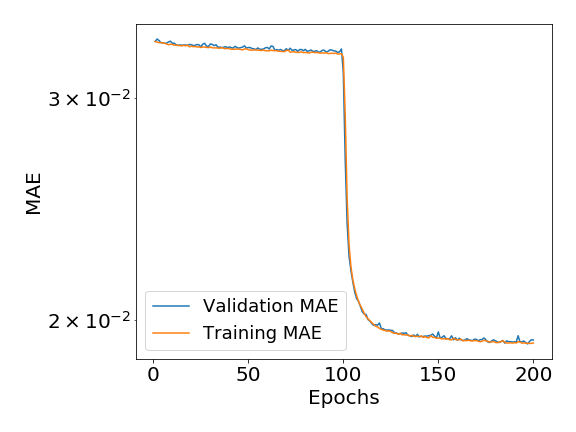
\includegraphics[width=1\textwidth]{figures/NN_training.png}
          \caption{Training and validation history of NN} 
          \label{fig:NN_training}
    \end{subfigure}%
    \begin{subfigure}{.46\textwidth}
          \centering
          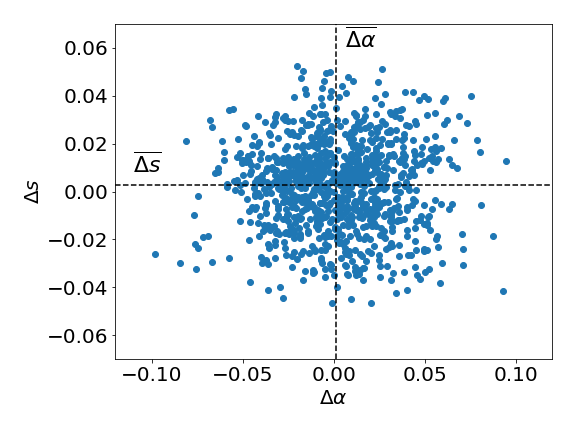
\includegraphics[width=1\textwidth]{figures/NN_error.png}
          \caption{Scatter plot of test errors in $\alpha$ and $s$}
    \label{fig:NN_errors}
    \end{subfigure}
    \caption{Training and validation history for NN, as well as a scatter plot of test errors in $\alpha$ and $s$. Note that no major overfitting is discernible, and that the errors seems to be uncorrelated.}
    \label{fig:NN}
\end{figure}



\subsection[Task 1]{Updating $h$ over multiple MCMC cycles in naive ABC}
\label{sec:result_h}

The empirically obtained updating scheme for $h$ that is used is given in equation \eqref{eq:emprical_h},

\begin{equation}
    \label{eq:emprical_h}
    h_{i+1} = \frac{h_i}{1+0.2\frac{\gamma_i}{\gamma_{i-1}}}.
\end{equation}
The goal of this updating scheme is to decrease $h$ at a rate that is governed by the change in acceptance ratio between cycles. We define the acceptance ratio to be the number of accepted $\alpha^*$ out of all proposed candidates. If the acceptance ratio decreases for cycle $i$ of MCMC as compared to the previous one, $\gamma_i>\gamma_{i-1}$, then $h$ will be decreased more than if $\gamma_i<\gamma_{i-1}$. Note that $h$ will never increase between cycles. Thus, $h$ will be decreased more if the acceptance ratio increases between cycles; this is because we expect the acceptance ratio to be artificially high for the early MCMC cycles, in which $h$ is too large. However, at some point, we expect that the obtained posterior, and thus the prior for the next cycle, converges towards the true posterior. When that happens, we desire an acceptance ratio that is close to one, since almost all of the candidates should be drawn from the true posterior. This scheme for updating $h$ does not reflect this behaviour, but the scheme can be extended by setting a minimum value for $h$. We opted for not doing this for simplicity, instead focusing on tuning the number of MCMC cycles.

\begin{figure}[ht]
    \centering
    \begin{subfigure}{.46\textwidth}
          \centering
          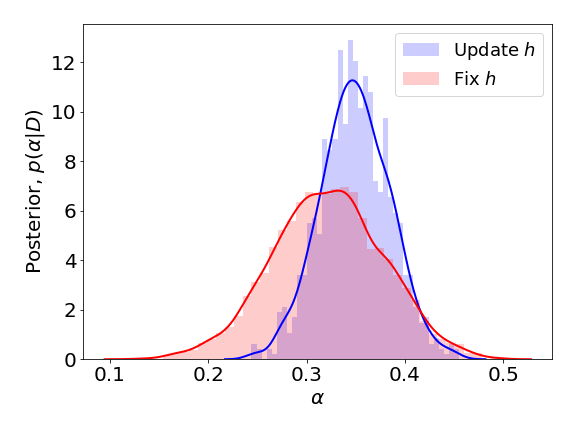
\includegraphics[width=1\textwidth]{figures/h_posterior.png}
          \caption{Posteriors for $\alpha$ after ten MCMC cycles} 
          \label{fig:h_posterior}
    \end{subfigure}%
    \begin{subfigure}{.46\textwidth}
          \centering
          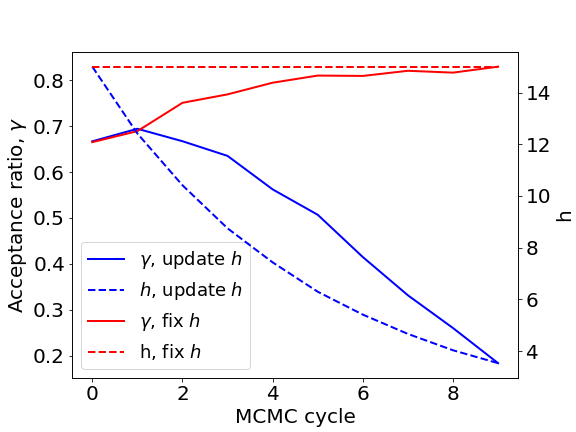
\includegraphics[width=1\textwidth]{figures/h_evolution.png}
          \caption{History over acceptance ratio and $h$}
    \label{fig:h_evolution}
    \end{subfigure}
    \caption{RMSE compared to the ground-truth PES as monitored during the training of the general-purpose GP, as well as predicted and ground-truth potential energy along the studied transition path.}
    \label{fig:h}
\end{figure}


The obtained posterior distributions after ten MCMC cycles with the Wasserstein distance, WSD, as a summary statistic and a uniform $\mathcal{U}(0, 0.5)$ initial prior for $\alpha$, either with a fixed value $h$ or with an $h$ that is updated for each cycle is given in figure \ref{fig:h_posterior}. The evolution of $h$ and the acceptance ratio for each of the two cases are given in figure \ref{fig:h_evolution}. We observe that the posterior for the case of updating $h$ is not as broad as when using a fixed $h$. Furthermore, studying the trace over the acceptance ratio in figure \ref{fig:h_evolution}, we see that the acceptance ratio decreases over the MCMC cycles when $h$ is decreased, as compared to the increasing acceptance ratio when $h$ is fixed. These results thus indicates that updating $h$ according to our scheme leads to a more restrictive acceptance of candidates for $\alpha$, which decreases the confidence interval. We will thus use this scheme for updating $h$ in the following sections.


\subsection[Task 1]{Comparison of summary statistics in naive ABC}
\label{sec:result_comp_sum_stat}

In this section we compare six different choices for eight different summary statistics: Kullblack-Leibler divergence (KL), Wasserstein distance (WSD), energy distance (ED) the L2 distance between the distributions (L2), the difference between the mean of the distributions (MEAN), the difference in standard deviation (STD), the combined mean and standard deviation difference (MEAN+STD), and using the neural network (NN). We are primarily interested in two aspects of these summary statistics. Firstly, do they capture the information necessary to infer $\alpha$? This can be seen in what value of $\alpha$ the respective posteriors converge to; if all summary statistics converge to the same $\alpha$, then they probably encode similar information. Secondly, we are interested in how the summary statistics affect the convergence speed. This can be seen from the size of the confidence interval (CI) after the same number of MCMC cycles. 

\begin{table}[h]
    \centering
    \caption{Obtained mean prediction for $\alpha$ together with a one standard deviation CI after ten MCMC cycles for the eight different summary statistics.}
    \begin{tabular}{||c c c c ||} 
         \hline
         KL & WSD & ED & L2   \\ [0.5ex] 
         \hline
         $0.318 +- 0.033$ & $0.309 +- 0.044$ & $0.308 +- 0.047$ & $0.288 +- 0.052$  \\ [0.5ex]
         \hline
         MEAN & STD & MEAN+STD & NN   \\
         \hline
         $0.258 +- 0.052$ & $0.323 +- 0.023$ & $0.323 +- 0.019$ & $0.336 +- 0.017$  \\ [0.5ex]
         \hline
    \end{tabular}
    \label{tab:sum_stat}
\end{table}

The mean and a confidence interval of one standard deviation for each of the summary statistics after ten MCMC cycles is given in table \ref{tab:sum_stat}. The empirical scheme for updating $h$ in equation \eqref{eq:emprical_h} was used, with the initial $h$ adjusted for each summary statistic. We observe that all summary statistics converge to roughly the same region, $\alpha \sim 0.3$, except for MEAN. This indicates that comparing the mean of the simulated and experimental distributions does not contain enough information on $\alpha$ for an accurate inference. As noted in the methodology, this could be due to $\alpha$ possibly affecting the spread of the distribution, which is further indicated by the standard deviation and the combined mean and standard deviation as summary statistics yielding better results, having the third and second smallest CI out of all studied statistics. However, the standard deviation as an information carrier of $\alpha$ may break down when $s$ becomes large, since this will skew the output distribution from the Galton board to one side. This could be a possible explanation as to why using the NN as a summary statistic yields the smallest confidence interval after ten MCMC cycles, since the NN is trained on this specific problem to extract information on $\alpha$ and $s$, regardless of $s$. The use of the NN is thus a problem specific statistic, as compared to the others which are all general. This also introduces direct dependence of the result on the neural network, which is not the case when we only use it to eliminate the latent variable. Thus, if one is to use the neural network, one should be careful when training and evaluating the network so that its limitations and biases are known. We will use the NN as a summary statistic in the following sections, due to it outperforming all of our other candidates.

\subsection{Sampling the posterior using naive ABC}
\label{sec:naive_posterior}
We have now seen how we can update $h$ for each MCMC cycle and which summary statistic gives the best performance so we are now in a position to perform a real sampling of the posterior. In figure \ref{fig:naive_posterior} we see the sampled posterior after one, six and ten MCMC cycles, when we used data set of 1000 experiments and 1000 proposed samples for each datum. We see that all three distribution are well sampled and approximate Gaussian indicating convergence as close to the posterior as the $h$ allows for. In figure \ref{fig:naive_evolution} the mean of the sampled approximate posterior together with a one standard deviation band is plotted. It is clear that the mean of the distribution don't change significantly but the width of it decreases. Even though it we may get a slightly smaller standard deviation if we perform more MCMC-cycles, decreasing $h$ further, the sampling has to a large extent converged to the true posterior. The mean posterior prediction of the infered $\alpha$ parameter is thus $0.346\pm 0.013$, with the one standard deviation uncertainty, and a 90 \% confidence interval is given by $[0.32, 0.37]$. We have over and over pointed out how we need to be careful doing inference aided by a neural network. From validating the neural network we now that in doing prediction we have a mean absolute error of approximately 0.02 for $\alpha$. This means that when we calculate the summary statistic it ought to have a hard time distinguish between simulated and observed data that is generated from $\alpha$'s with smaller difference then this. This may be one reason for why we don't keep decreasing the CI when lowering $h$, the approximation of the posterior is bounded by how well our summary statistic can differentiate $y$ from $y_{obs}$. 
\begin{figure}[H]
    \centering
    \begin{subfigure}{.46\textwidth}
          \centering
          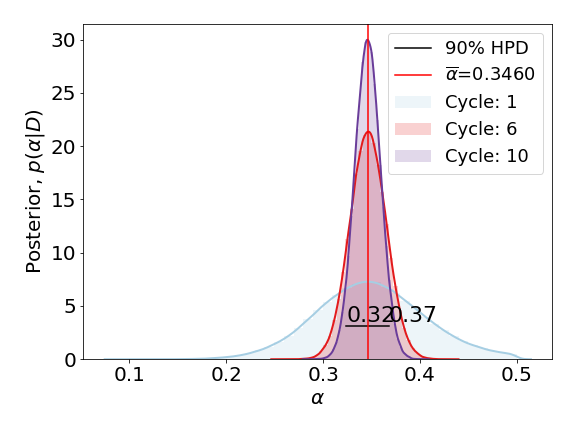
\includegraphics[width=1\textwidth]{figures/naive_posterior.png}
          \caption{Posteriors for $\alpha$ after ten MCMC cycles} 
          \label{fig:naive_posterior}
    \end{subfigure}%
    \begin{subfigure}{.46\textwidth}
          \centering
          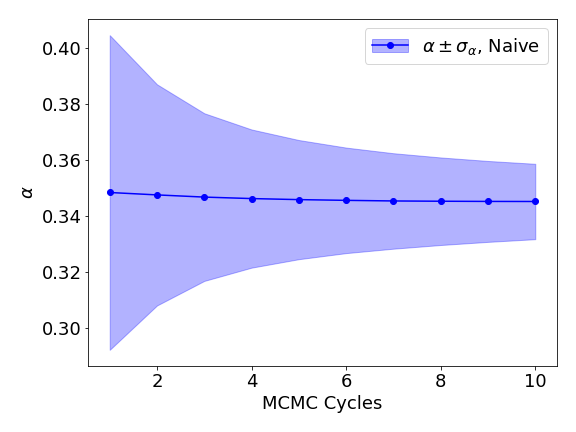
\includegraphics[width=1\textwidth]{figures/naive_ci.png}
          \caption{Evolution of CI over the ten MCMC cycles}
    \label{fig:naive_evolution}
    \end{subfigure}
    \caption{Caption}
    \label{fig:naive}
\end{figure}


\subsection[Task 4]{Improved data handling for ABC}
\label{sec:result_advanced}
We now turn to our improvements for the data handling in the naive ABC algorithm to try to decrease the CI presented in the previous section further. The improved data handling consists of two parts: interpreting all data points as data set $\hat{D}$, and an updated NN summary statistic that compares the experimental data set $\hat{D}$ to the simulated one $D$. As we shall see, the results indicate that the use of this summary statistics let us bypass the limitation of the summary statistic used in the naive approach, which combined with the more restrictive sampling due to the data set interpretation helps us decrease the CI further.  

Let us begin by briefly discussing the naive use of data, in which the ABC algorithm is simply repeated over multiple observed data $y_{obs}$. The obtained posterior distributions in the case of 1, 10, 100 and 1000 observed data points, after 10 MCMC cycles and with an initial uniform prior and the NN as a summary statistic, are given in figure \ref{fig:data_naive}. The number of proposed $\alpha$ was set so that the different cases for the number of data points would yield roughly the same number of considered candidates $\alpha^*$: for one data point we used 10 000 candidates, for 10 data points we used 1000 candidates for each data point etc. We observe that the width of the posterior is roughly the same regardless of the number of datum. This contradicts the intuition that the confidence interval should decrease when one adds more data. Instead, this naive approach to adding data seems to instead yield an averaging of the posteriors for the different observed data points. Another possible explanation as to why the width does not decrease as we add more data could be that we are limited by the uncertainty in the summary statistic, as discussed in section \ref{sec:naive_posterior}.

\begin{figure}[ht]
    \centering
    \begin{subfigure}{.46\textwidth}
          \centering
          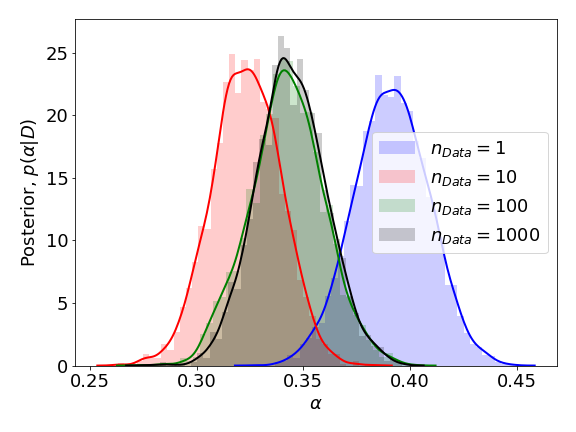
\includegraphics[width=1\textwidth]{figures/data_naive.png}
          \caption{Naive data approach} 
          \label{fig:data_naive}
    \end{subfigure}%
    \begin{subfigure}{.46\textwidth}
          \centering
          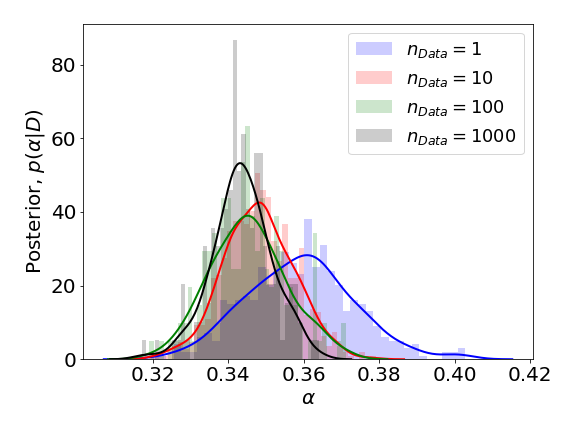
\includegraphics[width=1\textwidth]{figures/data_improved.png}
          \caption{Improved data approach}
    \label{fig:data_improved}
    \end{subfigure}
    \caption{Obtained posteriors after ten MCMC cycles for various numbers of data points $y_{obs}$, either in the case of the naive or the improved data approach.}
    \label{fig:data}
\end{figure}

These results can be contrasted with the obtained posterior when we instead interpret the multiple data points as a data set $D$, which are given in figure \ref{fig:data_improved}. We observe that the posteriors are not as wide overall as in the naive case, and that the width decreases when going from one datum to ten datum; for more data the difference is not discernible from the figure though. This could be due to us being limited by the improved summary statistic for more datum in this case as well. We will discuss this summary statistic in more detail in the next section. Nevertheless, this combination of interpreting the data as a data set, with the summary statistic to handle it, helps us decrease the CI past what we are able to achieve with the naive approach.


%Although both approaches uses the NN, in the naive approach we calculate the RMSE between the prediction for an observed $y_{obs}$ and a simulated $y(\alpha^*)$ for some candidate $\alpha^*$, whilst in the improved approach we calculate the mean $\alpha$ over the predictions for the observed data set $D$ and compare it to the mean $\alpha$ over the predictions of the simulated data set $\hat{D}$ for a candidate $\alpha^*$. We observed this summary statistic to yield a smaller CI than to calculate e.g. the RMSE over $D$ and $\hat{D}$, presumably because

\subsection{Sampling the posterior using improved ABC}

%Finally, we can combine these two strategies, the naive but quicker and the improved but slower approach to handling data, to obtain a final inference result for $\alpha$. To this end, we ran 10 cycles of MCMC using the naive approach, to yield a fairly converged posterior that we then could feed into the improved approach, after which we performed 10 MCMC cycles with the improved ABC algorithm. For both methods, we used the same 1000 data points $y_{obs}$ and used the neural network as a summary statistic. For each MCMC cycle, 1000 candidates where proposed for each data point $y_{obs}$ in the case of the naive approach, and for the case of the improved data handling 1000 candidates where proposed for the whole data set (i.e. one proposed candidate $\alpha^*$ per observed data $y_{obs}$ in $D$). The evolution of the mean of the posterior for $\alpha$, together with a one standard deviation CI, as a function of MCMC cycles is given in figure \ref{fig:ABC_final}. We observe that the CI decreases monotonously, and that it decreases more rapidly using the improved data handling scheme. The final one standard deviation CI for $\alpha$ after 20 MCMC cycles is $\alpha = 0.346 \pm 0.001$.

Finally we can perform the sampling with our improved method. For this we used the same data set that was used for the naive approach and used the naive posterior as prior. 10 MCMC cycles was performed where 1000 proposals for $\alpha$ was made in each cycle. The result is presented in figure \ref{}, which shows how the sampling the mean and one standard deviation uncertainty evolves
over the cycles. We can clearly see that the uncertainty decreases when we use compared to the naive approach and we still have a well sampled posterior. The final mean prediction of $\alpha$ is then $\alpha = 0.346 \pm 0.001$ with one standard deviation uncertainty and a 90 \% confidence interval is given by $[??, ??]$. This thus seems to be very successfull since we have significantly decreased the CI, but before we can draw some conclusions we must investigate if the choice of a different summary statistic gives rise to some new errors. For the naive approach concluded suspected that the uncertainty in the NN prediction limited us in how well we could determine $\alpha$, for the improved method we take a mean over different predictions so this uncertainty should decrease. As we saw in the section \ref{sec:validate_NN} this is true but when we get down to these uncertainties we discover a small bias in the network. This means that the mean of the errors in 1000 predicted $\alpha$'s is -0.002. Does this mean our one standard deviation of 0.001 indicate that we are way to certain about the inference? Well not necessarily, because this bias gets applied both to the simulated data set and the experimental one and thus ought to cancel out. What is more interesting is how much the bias varies for different data set, and as we saw in \ref{sec:validate_NN} the standard deviation of the mean predictive $\alpha$ errors is 0.001. As for the naive approach the summary statistic would have a hard time differentiate between two data set generated with a $\alpha$ with smaller difference than $\alpha$ which we see is the final standard deviation in our posterior. 







\printbibliography

\end{document}
